% !TeX root = ../example.tex

\chapter{图表示例}

\section{插图}

图片通常在 \env{figure} 环境中使用 \cs{includegraphics} 插入,如图~\ref{fig:example} 的源代码。
建议矢量图片使用 PDF 格式,比如数据可视化的绘图;
照片应使用 JPG 格式;
其他的栅格图应使用无损的 PNG 格式。
注意,LaTeX 不支持 TIFF 格式;EPS 格式已经过时。

\begin{figure}
  \centering
  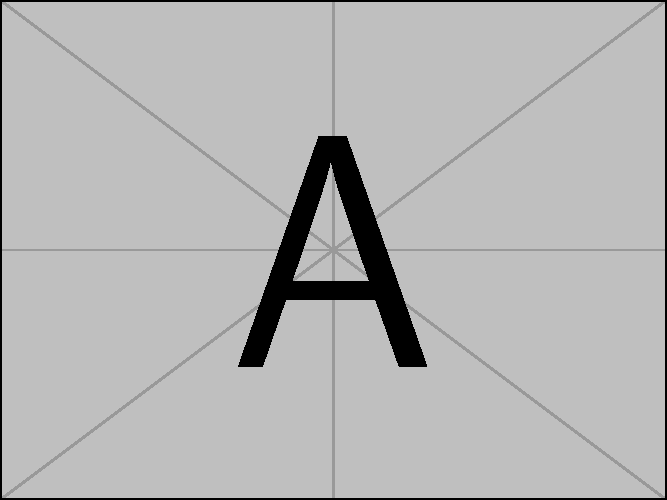
\includegraphics[width=0.6\linewidth]{example-image-a.pdf}
  \bicaption{示例图片}{Example figure}
  \label{fig:example}
\end{figure}

图包括曲线图、构造图、示意图、框图、流程图、记录图、照片等。
图应具有自明性,一般随文编排,先文字后见图。
图中各部分说明应采用中文(引用的外文图除外)或数字符号,各项文字说明置于图下图题之上。


图序与图题:图序即图的编号,由“图”和阿拉伯数字组成,较多时可按章依序编号,如图 1-1、图 1-2。图题即图的名称,置于图序之后,图序和图题间
空 1 个字符,中英文对照,居中置于图的下方,中文在上。该模板中使用 \pkg{bicaption} 宏包实现双语图题。如有分图时,分图号用(a)、(b)表示,分图题置于分图之下或图题之下。如放在图题之下,多个分图题之间用“;”隔开,\emph{末尾不加句点}。
引用文献中的图时,除在正文中标注参考文献序号以外,还必须在中、英文图题的右上角标注参考文献序号。
推荐使用 \pkg{subfig} 宏包来处理, 比如图~\subref*{fig:subfig-a} 和图~\subref*{fig:subfig-b}。

若图或表中有附注,采用英文小写字母顺序编号,附注写在图或表的下方。
% LaTeX 传统上一般将附注的内容同图表的标题写在一起,形成很长的一段文字。

如论文中图表较多,可以分别列出清单置于目录页之后。图的清单应有序号、图题和页码。表的清单应有序号、表题和页码。

\begin{figure}
  \centering
  \subfloat[分图 A\label{fig:subfig-a}]
    {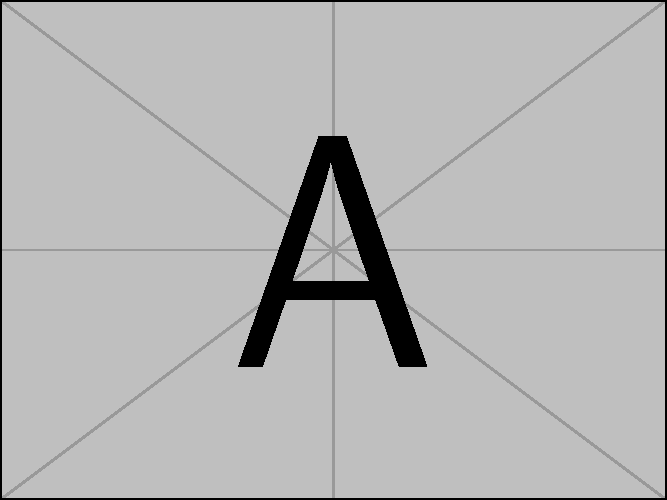
\includegraphics[width=0.4\linewidth]{example-image-a.pdf}}
  \subfloat[分图 B\label{fig:subfig-b}]
    {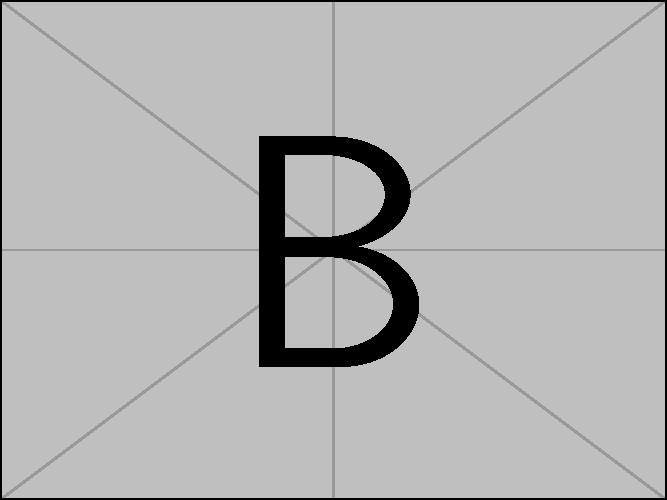
\includegraphics[width=0.4\linewidth]{example-image-b.pdf}}
  \bicaption[多个分图的示例]{% 总图题写在方括号内,其显示在插图列表中
  	多个分图的示例:(a) 左图;(b) 右图
  }{
  	Multiple subfigure example:
  	(a) figure on the left; (b)	figure on the right
  }
  \label{fig:multi-image}
\end{figure}



\section{表格}

表应具有自明性。为使表格简洁易读,尽可能采用三线表,如表~\ref{tab:three-line}。
三条线可以使用 \pkg{booktabs} 宏包提供的命令生成。

\begin{table}[!htb]
  \centering
  \bicaption{三线表示例}{Table with three rules}
  \begin{tabular}{ll}
    \toprule
    文件名          & 描述                         \\
    \midrule
    thuthesis.dtx   & 模板的源文件,包括文档和注释 \\
    thuthesis.cls   & 模板文件                     \\
    thuthesis-*.bst & BibTeX 参考文献表样式文件    \\
    thuthesis-*.bbx & BibLaTeX 参考文献表样式文件  \\
    thuthesis-*.cbx & BibLaTeX 引用样式文件        \\
    \bottomrule
  \end{tabular}
  \label{tab:three-line}
\end{table}

表格如果有附注,尤其是需要在表格中进行标注时,可以使用 \pkg{threeparttable} 宏包。

\begin{table}[!htb]
  \centering
  \begin{threeparttable}[c]
    \bicaption{带附注的表格示例}{Table example with notes}
    \label{tab:three-part-table}
    \begin{tabular}{ll}
      \toprule
      文件名                 & 描述                         \\
      \midrule
      thuthesis.dtx\tnote{a} & 模板的源文件,包括文档和注释 \\
      thuthesis.cls\tnote{b} & 模板文件                     \\
      thuthesis-*.bst        & BibTeX 参考文献表样式文件    \\
      thuthesis-*.bbx        & BibLaTeX 参考文献表样式文件  \\
      thuthesis-*.cbx        & BibLaTeX 引用样式文件        \\
      \bottomrule
    \end{tabular}
    \begin{tablenotes}
      \item [a] 可以通过 xelatex 编译生成模板的使用说明文档;
        使用 xetex 编译 \file{thuthesis.ins} 时则会从 \file{.dtx} 中去除掉文档和注释,得到精简的 \file{.cls} 文件。
      \item [b] 更新模板时,一定要记得编译生成 \file{.cls} 文件,否则编译论文时载入的依然是旧版的模板。
    \end{tablenotes}
  \end{threeparttable}
\end{table}

如某个表需要转页接排,可以使用 \pkg{longtable} 宏包,需要在随后的各页上重复表的编号。
编号后跟表题(可省略)和“(续)”,置于表上方。续表均应重复表头。

\begin{longtable}{cccc}
	\bicaption{跨页长表格的表题}{Longtable example} \\
	\toprule
	表头 1 & 表头 2 & 表头 3 & 表头 4 \\
	\midrule
	\endfirsthead
	\bicaption[]{跨页长表格的表题(续)}{Longtable example(continue)} \\
	\toprule
	表头 1 & 表头 2 & 表头 3 & 表头 4 \\
	\midrule
	\endhead
	\bottomrule
	\endfoot
	Row 1  & & & \\
	Row 2  & & & \\
	Row 3  & & & \\
	Row 4  & & & \\
	Row 5  & & & \\
	Row 6  & & & \\
	Row 7  & & & \\
	Row 8  & & & \\
	Row 9  & & & \\
	Row 10 & & & \\
	Row 11 & & & \\
	Row 12 & & & \\
	Row 13 & & & \\
	Row 14 & & & \\
	Row 15 & & & \\
	Row 16 & & & \\
	Row 17 & & & \\
	Row 18 & & & \\
	Row 19 & & & \\
	Row 20 & & & \\
	Row 21 & & & \\
	Row 22 & & & \\
	Row 23 & & & \\
	Row 24 & & & \\
	Row 25 & & & \\
	Row 26 & & & \\
	Row 27 & & & \\
	Row 28 & & & \\
	Row 29 & & & \\
	Row 30 & & & \\
	Row 31 & & & \\
	Row 32 & & & \\
	Row 33 & & & \\
	Row 34 & & & \\
	Row 35 & & & \\
	Row 36 & & & \\
	Row 37 & & & \\
	Row 38 & & & \\
	Row 39 & & & \\
	Row 40 & & & \\
	Row 41 & & & \\
	Row 42 & & & \\
	Row 43 & & & \\
	Row 44 & & & \\
	Row 45 & & & \\
	Row 46 & & & \\
	Row 47 & & & \\
	Row 48 & & & \\
	Row 49 & & & \\
	Row 50 & & & \\
\end{longtable}

算法可以使用\pkg{algorithm}、\pkg{algorithmicx}、\pkg{algpseudocode}等宏包实现。欧几里得算法过程如算法~\ref{euclid}所示。
\begin{algorithm}[!htb]
	\caption{欧几里得算法}
	\label{euclid}
	\begin{algorithmic}[1]
		\Require 两个正整数$a$, $b$
		\Ensure 最大公约数
		\Procedure{Euclid}{$a,b$}\Comment{$a$ 和 $b$ 的最大公约数}
		\State $r \gets a \bmod b$
		\While{$r \not= 0$}\Comment{若$r$为0,则直接返回}
		\State $a \gets b$
		\State $b \gets r$
		\State $r \gets a \bmod b$
		\EndWhile\label{euclidendwhile}
		\State \textbf{return} $b$\Comment{最大公约数为$b$}
		\EndProcedure
	\end{algorithmic}
\end{algorithm}